% TikZ redraw for exercise 4-5
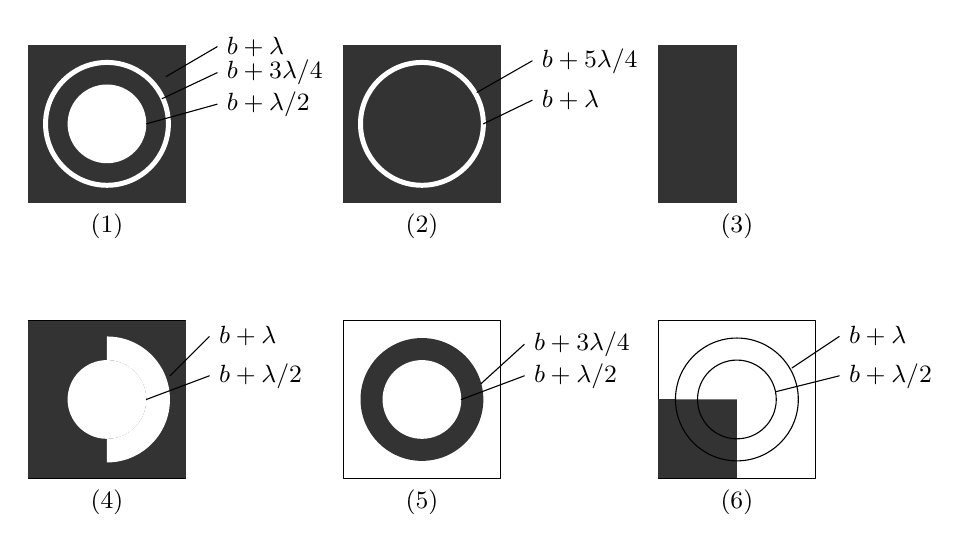
\begin{tikzpicture}[font=\small,line cap=round,line join=round]
\foreach\x/\y/\k in {0/0/1,4/0/2,8/0/3,0/-3.5/4,4/-3.5/5,8/-3.5/6}{\begin{scope}[shift={(\x,\y)}]\draw(-1,-1)rectangle(1,1);\ifnum\k<5\fill[black!80](-1,-1)rectangle(1,1);\fi
\ifcase\k\or\fill[white](0,0)circle(.5);\draw[white,line width=1.8pt](0,0)circle(.78);\draw(.5,0)--(1.4,.25)node[right]{$b+\lambda/2$};\draw(.7,.32)--(1.4,.65)node[right]{$b+3\lambda/4$};\draw(.75,.6)--(1.4,.98)node[right]{$b+\lambda$};
\or\draw[white,line width=1.8pt](0,0)circle(.78);\draw(.78,0)--(1.4,.3)node[right]{$b+\lambda$};\draw(.7,.4)--(1.4,.8)node[right]{$b+5\lambda/4$};
\or\fill[white](0,-1)rectangle(1,1);
\or\fill[white](0,0)circle(.5);\fill[white](0,-.8)arc(-90:90:.8)--(0,.5)arc(90:-90:.5)--cycle;\draw(.5,0)--(1.3,.3)node[right]{$b+\lambda/2$};\draw(.8,.3)--(1.3,.8)node[right]{$b+\lambda$};
\or\fill[black!80](0,0)circle(.78);\fill[white](0,0)circle(.5);\draw(.5,0)--(1.3,.3)node[right]{$b+\lambda/2$};\draw(.75,.2)--(1.3,.7)node[right]{$b+3\lambda/4$};
\or\fill[black!80](-1,-1)rectangle(0,0);\fill[white](0,0)circle(.78);\fill[black!80](0,0)--(-.78,0)arc(180:270:.78)--cycle;\fill[white](0,0)circle(.5);\fill[black!80](0,0)--(-.5,0)arc(180:270:.5)--cycle;\draw(0,0)circle(.78);\draw(0,0)circle(.5);\draw(.5,.1)--(1.3,.3)node[right]{$b+\lambda/2$};\draw(.7,.4)--(1.3,.8)node[right]{$b+\lambda$};\fi\node at(0,-1.3){(\k)};\end{scope}}
\end{tikzpicture}
